% Página
\section{Confidencialidade}

A Confidencialidade refere-se à garantia de que as informações são acessíveis apenas por pessoas autorizadas. Em outras palavras, é a proteção contra a divulgação não autorizada de dados. Este pilar é essencial para manter a privacidade dos dados pessoais e sensíveis, como informações financeiras, médicas ou estratégicas de uma organização. Técnicas de criptografia são amplamente utilizadas para garantir a confidencialidade, assegurando que, mesmo que os dados sejam interceptados, eles não possam ser lidos ou compreendidos por indivíduos não autorizados.

\subsection{Algoritmo Simétrico}

Entre os diversos tipos de algoritmos de criptografia, o algoritmo de criptografia simétrica é um dos mais comuns e amplamente utilizados. Neste tipo de algoritmo, a mesma chave(K) é utilizada tanto para criptografar(C), gerando a mensagem cifrada(M), quanto para descriptografar(D) os dados, gerando o Texto Plano(T).\\

A Figura \ref{fig:algoritmo_simetrico} ilustra o funcionamento do algoritmo de criptografia simétrica. Para mostrar o funcionamento do algoritmo, vamos considerar três personagens: \textbf{Alice}, \textbf{Bob} e \textbf{Eva}. Alice e Bob desejam se comunicar de forma segura, enquanto Eva deseja ler a mensagem trocadas entre eles.

\begin{figure}[H]
	\centering
	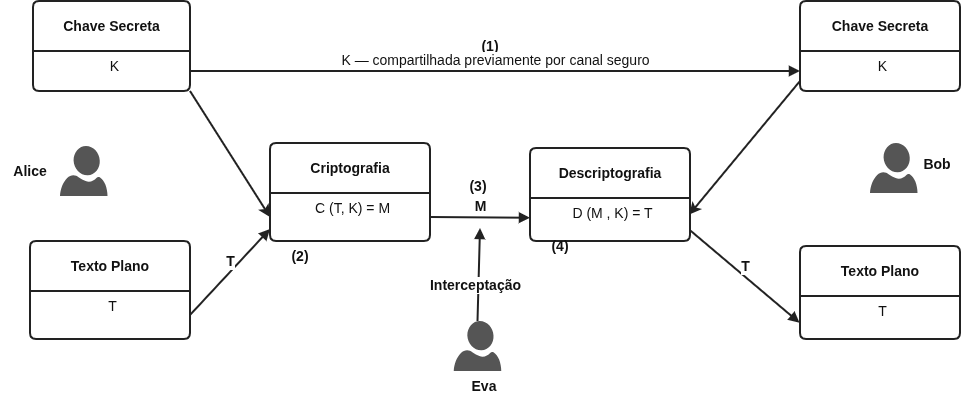
\includegraphics[scale=0.45]{algoritmo_simetrico.png}
	\caption{Funcionamento do algoritmo de criptografia simétrico}
	\label{fig:algoritmo_simetrico}
\end{figure}

\pagebreak
\textbf{Funcionamento do Algoritmo de Criptografia Simétrico}

\begin{enumerate}
	\item Alice e Bob precisam obter a mesma chave secreta (K) por um mecanismo seguro antes de trocar mensagens. O comando abaixo gera uma chave aleatória de 256 bits para o exemplo; executá-lo em Alice não entrega automaticamente uma cópia a Bob.
	\begin{tcolorbox}[width=\textwidth]
		{\normalsize
			\begin{verbatim}
			$ umask 077
			$ openssl rand -hex 32 > K.hex
			\end{verbatim}
		}
	\end{tcolorbox}
	\item Quando Alice deseja enviar o Texto Plano(T) para Bob, ela utiliza AES-256-CBC, a Chave Secreta(K) e um IV aleatório para gerar o Texto Cifrado(M). O IV não é secreto e deve acompanhar o texto cifrado; gere um IV novo e imprevisível para cada cifragem. Este exemplo demonstra apenas confidencialidade: em produção, prefira uma cifra autenticada (AEAD), como AES-GCM, ou combine CBC com um MAC usando uma chave independente e autentique o IV e o texto cifrado antes de decifrar.
	\begin{tcolorbox}[width=\textwidth]
		{\normalsize
			\begin{verbatim}
			$ IV_HEX=$(openssl rand -hex 16)
			$ printf '%s' "$IV_HEX" > M.iv
			$ openssl enc -aes-256-cbc -K "$(cat K.hex)" -iv "$IV_HEX" \
			  -in T.txt -out M.enc
			\end{verbatim}
		}
	\end{tcolorbox}
	\item Alice envia o Texto Cifrado(M) e o IV para Bob através de um canal de comunicação inseguro. Se Eva apenas interceptar esses dados e a chave permanecer secreta, ela não deverá conseguir recuperar a mensagem original. Como CBC sozinho não autentica os dados, um atacante ativo ainda pode alterar o texto cifrado ou o IV sem que a alteração seja detectada de forma confiável.
	\item Ao receber o Texto Cifrado(M), Bob utiliza o mesmo algoritmo de Descriptografia(D) e a Chave Secreta(K) para transformar o Texto Cifrado(M) de volta ao Texto Plano(T).
	\begin{tcolorbox}[width=\textwidth]
		{\normalsize
			\begin{verbatim}
			$ openssl enc -d -aes-256-cbc -K "$(cat K.hex)" -iv "$(cat M.iv)" \
			  -in M.enc -out T.txt
			\end{verbatim}
		}
	\end{tcolorbox}
\end{enumerate}

A principal vantagem dos algoritmos de criptografia simétrica é sua eficiência e velocidade, especialmente em comparação com os algoritmos de criptografia assimétrica. No entanto, Alice e Bob precisam estabelecer a chave secreta com segurança. Se Eva descobrir essa chave, poderá decifrar as mensagens protegidas por ela.\\

Esses comandos são didáticos: o arquivo K.hex contém a chave em claro, e a opção \texttt{-K} passa a chave como argumento do processo, onde ela pode ficar visível durante a execução. Em produção, use uma biblioteca criptográfica e um mecanismo de armazenamento e uso de chaves que evitem essa exposição. Alice e Bob podem provisionar a chave por um canal protegido ou estabelecê-la por um protocolo autenticado de acordo de chaves.\\

\subsection{Algoritmo Assimétrico}

O algoritmo de criptografia assimétrica é uma técnica fundamental no campo da segurança e criptografia. Diferente dos algoritmos de criptografia simétrica, que utilizam a mesma chave para criptografar e descriptografar os dados, os algoritmos assimétricos usam um par de chaves: uma chave pública(KPu) e uma chave privada(KPr). Vamos explorar o funcionamento desse algoritmo através dos personagens Alice, Bob e Eva exemplificado pela Figura \ref{fig:algoritmo_assimetrico}.

\begin{figure}[H]
	\centering
	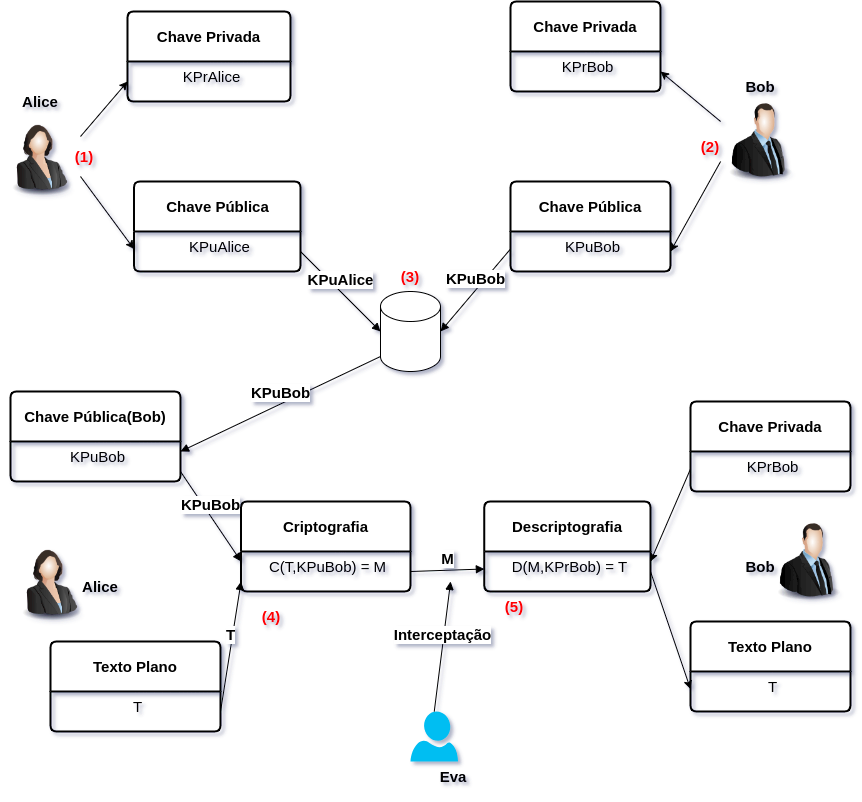
\includegraphics[scale=0.45]{algoritmo_assimetrico.png}
	\caption{Funcionamento do algoritmo de criptografia assimétrico}
	\label{fig:algoritmo_assimetrico}
\end{figure}

\pagebreak

\textbf{Funcionamento do Algoritmo de Criptografia Assimétrico}

\begin{enumerate}
	\item Alice gera um par de chaves, Chave Pública(KPuAlice) e Chave Privada(KPrAlice);
	\begin{tcolorbox}[width=\textwidth]
		{\normalsize
			\begin{verbatim}
			$ openssl genpkey -algorithm RSA -out KPrAlice.pem -pkeyopt rsa_keygen_bits:2048
			$ openssl rsa -pubout -in KPrAlice.pem -out KPuAlice.pem
			\end{verbatim}
		}
	\end{tcolorbox}
	\item Bob gera um par de chaves, Chave Pública(KPuBob) e Chave Privada(KPrBob);
	\begin{tcolorbox}[width=\textwidth]
		{\normalsize
			\begin{verbatim}
			$ openssl genpkey -algorithm RSA -out KPrBob.pem -pkeyopt rsa_keygen_bits:2048
			$ openssl rsa -pubout -in KPrBob.pem -out KPuBob.pem
			\end{verbatim}
		}
	\end{tcolorbox}
	\item Tanto Alice quanto Bob enviam as suas respectivas chaves públicas, KPuAlice e KPuBob, para um servidor de chave pública;
	\item Antes de usar a chave pública recuperada do servidor, Alice deve verificar por um meio confiável que ela realmente pertence a Bob, por exemplo, validando um certificado digital ou comparando sua impressão digital por um canal autenticado. A presença da chave no servidor, por si só, não comprova essa associação: um atacante que substitua a chave de Bob pela sua própria pode interceptar a comunicação;
	\item Quando Alice deseja enviar um Texto Plano (T) curto para Bob, ela utiliza a Chave Pública do Bob (KPuBob.pem) para gerar o Texto Cifrado (M). Com RSA de 2048 bits e OAEP/SHA-256, a entrada deve ter no máximo 190 bytes. Para mensagens maiores, usa-se criptografia híbrida: Alice cifra a mensagem com uma chave simétrica aleatória usando uma cifra autenticada, como AES-GCM, e cifra essa chave simétrica com a chave pública de Bob.
	\begin{tcolorbox}[width=\textwidth]
		{\normalsize
			\begin{verbatim}
			$ openssl pkeyutl -encrypt -inkey KPuBob.pem -pubin -in T.txt -out M.bin \
			  -pkeyopt rsa_padding_mode:oaep -pkeyopt rsa_oaep_md:sha256
			\end{verbatim}
		}
	\end{tcolorbox}
	\item Ao receber o Texto Cifrado(M), o Bob utiliza sua Chave Privada(KPrBob) para descriptografá-la obtendo o Texto Plano(T).
	\begin{tcolorbox}[width=\textwidth]
		{\normalsize
			\begin{verbatim}
			$ openssl pkeyutl -decrypt -inkey KPrBob.pem -in M.bin -out T.txt \
			  -pkeyopt rsa_padding_mode:oaep -pkeyopt rsa_oaep_md:sha256
			\end{verbatim}
		}
	\end{tcolorbox}
\end{enumerate}

Se Alice usar uma chave pública de Bob cuja associação com ele foi verificada, e Bob proteger sua chave privada, a cifragem com RSA-OAEP protege a confidencialidade contra Eva, mesmo que ela intercepte o texto cifrado. Esse fluxo, por si só, não comprova que a mensagem foi enviada por Alice: qualquer pessoa que conheça a chave pública de Bob pode cifrar mensagens para ele. Para autenticar a origem, Alice deve assinar a mensagem com sua chave privada, e Bob deve verificar a assinatura usando uma chave pública de Alice cuja associação também seja confiável.\\

Na criptografia híbrida, a cifra autenticada permite detectar alterações no conteúdo cifrado, mas não identifica quem o produziu. A assinatura digital fornece essa verificação de origem, desde que a chave pública do remetente esteja autenticada.

\subsection{Key-Encryption-Key (KEK)}

Uma Key-Encryption Key (KEK), ou chave de criptografia de chaves, é usada para proteger (encapsular) outras chaves. Neste exemplo, MKBob, derivada da Senha Mestra por uma KDF, exerce o papel de KEK: ela protege a DEK, que por sua vez cifra os dados. Essa separação facilita o gerenciamento e a troca de chaves, mas não garante segurança por si só.\\

A Figura \ref{fig:kek} ilustra a hierarquia de chaves: M1 é a DEK protegida pela KEK, e M2 são os dados protegidos pela DEK.

\begin{figure}[H]
	\centering
	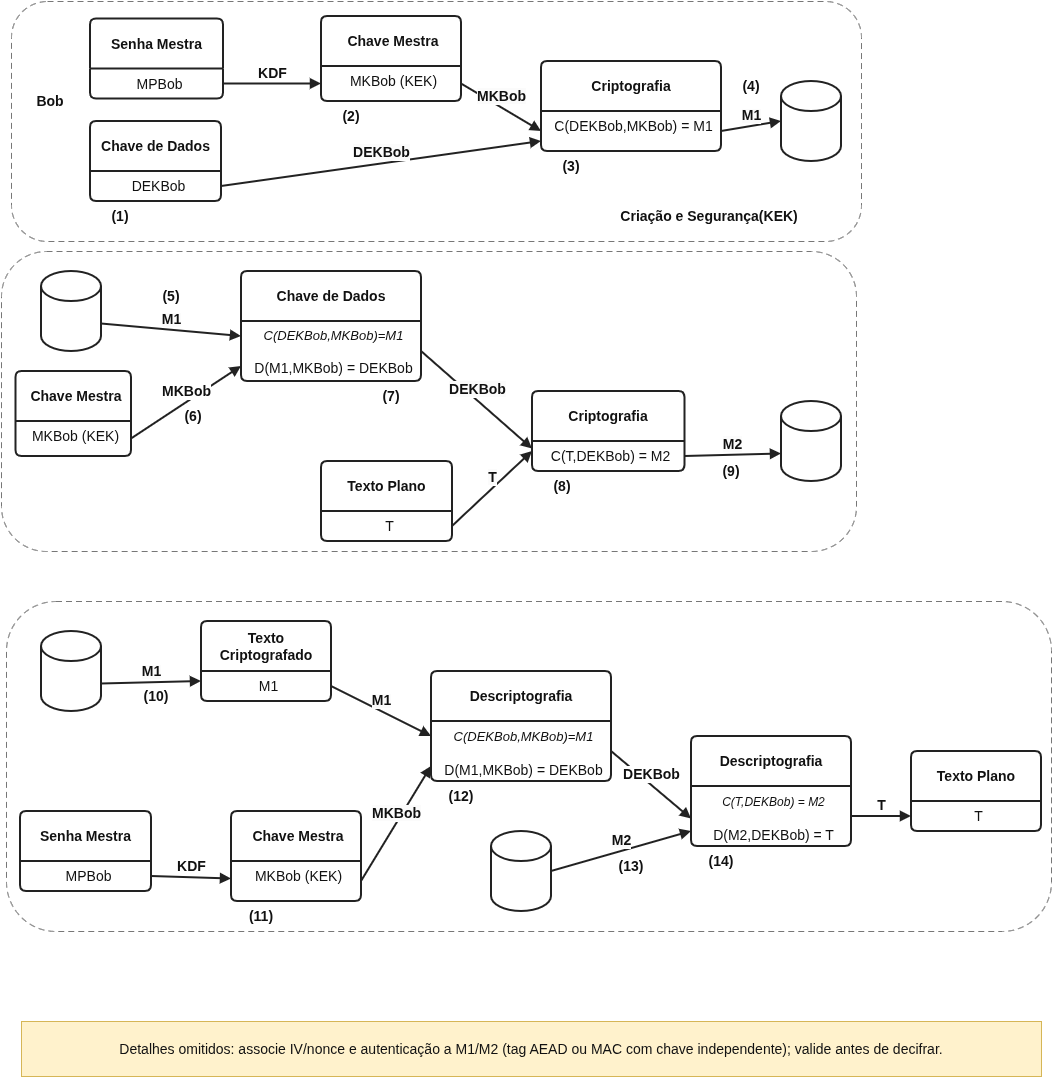
\includegraphics[scale=0.45]{kek.png}
	\caption{Funcionamento do conceito Key-Encryption-Key (KEK)}
	\label{fig:kek}
\end{figure}

\textbf{Nota sobre os comandos:} são exemplos didáticos e usam AES-CBC sem autenticação. Em produção, prefira AEAD para proteger M1 e M2; se CBC for necessário, use um MAC com chave independente que cubra o IV e o texto cifrado, e verifique-o antes de decifrar. Armazene com M1 seu IV, o salt e os parâmetros da KDF; armazene com M2 seu IV. A cópia de M1 permite tentativas offline de adivinhar a Senha Mestra, portanto a KDF não substitui uma senha forte. Os exemplos são didáticos e gravam material secreto em arquivos locais. O comando `openssl kdf` recebe a Senha Mestra como argumento de processo, e os comandos AES-CBC também passam a chave dessa forma; esses exemplos não devem ser usados assim em produção.

\textbf{- Criptografar a Chave de Dados(DEKBob)}

\begin{enumerate}
	\item Bob gera uma DEK aleatória de 256 bits;
	\begin{tcolorbox}[width=\textwidth]
		{\normalsize
			\begin{verbatim}
			$ set -o pipefail
			$ umask 077
			$ openssl rand -out DEKBob.bin 32
			\end{verbatim}
		}
	\end{tcolorbox}
	\item Bob deriva a KEK (MKBob.hex) a partir da Senha Mestra com PBKDF2-HMAC-SHA-256, 600.000 iterações e um salt aleatório de 16 bytes (128 bits). O salt e os parâmetros da KDF não são secretos e devem ser preservados para a recuperação;
	\begin{tcolorbox}[width=\textwidth]
		{\footnotesize
			\begin{verbatim}
			$ umask 077
			$ set -o pipefail
			$ if [ ! -s MKBob.salt ]; then openssl rand -hex 16 > MKBob.salt; fi
			$ SALT_HEX=$(cat MKBob.salt)
			$ read -rs MASTER_PASSWORD; printf '\n'
			$ printf 'PBKDF2-HMAC-SHA-256\niterations=600000\nkey_length=32\n' > MKBob.kdf
			$ openssl kdf -keylen 32 -kdfopt digest:SHA256 \
			  -kdfopt "pass:$MASTER_PASSWORD" -kdfopt "salt:$SALT_HEX" \
			  -kdfopt iter:600000 PBKDF2 | tr -d ':\n' > MKBob.hex.tmp \
			  && mv MKBob.hex.tmp MKBob.hex
			$ chmod 600 MKBob.salt MKBob.hex MKBob.kdf
			$ unset MASTER_PASSWORD
			\end{verbatim}
		}
	\end{tcolorbox}
	\item Bob protege (encapsula) a DEK com a KEK MKBob, gerando M1. O IV acompanha M1;
	\begin{tcolorbox}[width=\textwidth]
		{\scriptsize
			\begin{verbatim}
			$ IV_HEX=$(openssl rand -hex 16)
			$ printf '%s' "$IV_HEX" > M1.iv
			$ openssl enc -aes-256-cbc -K "$(cat MKBob.hex)" -iv "$IV_HEX" \
			  -in DEKBob.bin -out M1.enc
			\end{verbatim}
		}
	\end{tcolorbox}
	\item Bob envia M1, seu IV, o salt e os parâmetros da KDF para o servidor;
\end{enumerate}

\textbf{- Criptografar o Texto Plano(T) com uma Chave de Dados DEKBob}

\begin{enumerate}
	\setcounter{enumi}{4} % Define o contador para começar do número 5
	\item Bob recupera o Texto Cifrado M1 do servidor;
	\item Bob possui sua Chave Mestra (MKBob.hex);
	\item Bob descriptografa o Texto Cifrado M1 para obter acesso à sua Chave de Dados (DEKBob.bin);
	\begin{tcolorbox}[width=\textwidth]
		{\scriptsize
			\begin{verbatim}
			$ openssl enc -d -aes-256-cbc -K "$(cat MKBob.hex)" -iv "$(cat M1.iv)" \
			  -in M1.enc -out DEKBob.bin
			\end{verbatim}
		}
	\end{tcolorbox}
	\item Bob cifra o Texto Plano (T) com a DEK e um IV aleatório, gerando M2. O IV acompanha M2;
	\begin{tcolorbox}[width=\textwidth]
		{\small
			\begin{verbatim}
			$ DEK_HEX=$(od -An -v -tx1 DEKBob.bin | tr -d ' \n')
			$ IV_HEX=$(openssl rand -hex 16)
			$ printf '%s' "$IV_HEX" > M2.iv
			$ openssl enc -aes-256-cbc -K "$DEK_HEX" -iv "$IV_HEX" \
			  -in T.txt -out M2.enc
			\end{verbatim}
		}
	\end{tcolorbox}
	\item Bob envia M2 e seu IV para o servidor;
\end{enumerate}

\textbf{- Descriptografar o Texto Cifrado M2 para obter o Texto Plano(T)}

\begin{enumerate}
	\setcounter{enumi}{9} % Define o contador para começar do número 10
	\item Bob recupera o Texto Cifrado M1 do servidor;
	\item Bob possui sua Chave Mestra (MKBob.hex);
	\item Bob descriptografa o Texto Cifrado M1 com sua Chave Mestra (MKBob.hex) para obter acesso à sua Chave de Dados (DEKBob.bin);
	\begin{tcolorbox}[width=\textwidth]
		{\scriptsize
			\begin{verbatim}
			$ openssl enc -d -aes-256-cbc -K "$(cat MKBob.hex)" -iv "$(cat M1.iv)" \
			  -in M1.enc -out DEKBob.bin
			\end{verbatim}
		}
	\end{tcolorbox}
	\item Bob recupera o Texto Cifrado M2 do servidor;
	\item Bob descriptografa o Texto Cifrado M2 com sua Chave de Dados (DEKBob.bin) para obter acesso ao Texto Plano (T);
	\begin{tcolorbox}[width=\textwidth]
		{\small
			\begin{verbatim}
			$ DEK_HEX=$(od -An -v -tx1 DEKBob.bin | tr -d ' \n')
			$ openssl enc -d -aes-256-cbc -K "$DEK_HEX" -iv "$(cat M2.iv)" \
			  -in M2.enc -out T.txt
			\end{verbatim}
		}
	\end{tcolorbox}
\end{enumerate}

Uma KEK protege chaves de dados e ajuda a separar a gestão de chaves da cifragem dos dados. A confidencialidade e a detecção de alterações dependem também dos algoritmos, modos e metadados usados; a hierarquia KEK/DEK, sozinha, não garante integridade nem autenticidade.

\subsection{Key Derivation Functions (KDF)}

As funções de derivação de chaves (Key Derivation Functions -- KDFs) transformam um segredo inicial, como uma senha, em uma ou mais chaves criptográficas de tamanho definido. A Figura \ref{fig:kdf} ilustra a derivação de uma chave a partir de uma Senha Mestra. A derivação também depende de um salt e de parâmetros que controlam o custo da operação.

O salt deve ser único para cada derivação e pode ser armazenado junto aos dados e aos parâmetros da KDF; ele não precisa ser secreto. Seu uso evita que senhas iguais produzam necessariamente a mesma chave e dificulta o pré-cálculo de tabelas. Uma KDF apropriada para senhas aumenta o custo de cada tentativa de adivinhação, mas não elimina ataques de força bruta nem compensa uma senha fraca.

Um exemplo é PBKDF2 (Password-Based Key Derivation Function 2), especificada no PKCS \#5. Ela aplica uma função pseudorrandômica, como HMAC-SHA-256, repetidamente; o número de iterações é um de seus parâmetros de custo. Argon2, selecionada na Password Hashing Competition, é outra opção e permite configurar parâmetros como memória, tempo e paralelismo. Os parâmetros utilizados devem ser armazenados para possibilitar a derivação posterior da mesma chave e escolhidos conforme as recomendações atuais e os recursos disponíveis.

\begin{figure}[H]
\centering
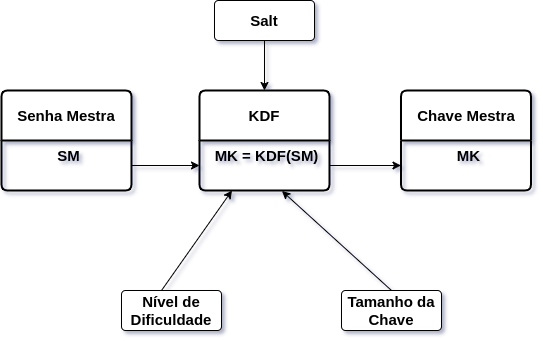
\includegraphics[scale=0.45]{kdf.png}
\caption{Derivação de chave a partir de uma senha, salt e parâmetros da KDF}
\label{fig:kdf}
\end{figure}
Os comandos a seguir usam o OpenSSL para derivar uma chave com PBKDF2-HMAC-SHA-256. Na primeira execução, geram e salvam um salt aleatório; nas seguintes, reutilizam o salt salvo para derivar novamente a mesma chave. O arquivo MKBob.kdf registra algoritmo, iterações e tamanho da chave.

\begin{enumerate}
	\item Derivar uma chave de 256 bits usando PBKDF2 e salvar sua representação hexadecimal localmente. O salt é armazenado junto dos metadados necessários à derivação.
	\begin{tcolorbox}[width=\textwidth]
	{\footnotesize
		\begin{verbatim}
			$ umask 077
			$ set -o pipefail
			$ if [ ! -s MKBob.salt ]; then openssl rand -hex 16 > MKBob.salt; fi
			$ SALT_HEX=$(cat MKBob.salt)
			$ read -rs MASTER_PASSWORD; printf '\n'
			$ printf 'PBKDF2-HMAC-SHA-256\niterations=600000\nkey_length=32\n' > MKBob.kdf
			$ openssl kdf -keylen 32 -kdfopt digest:SHA256 \
			  -kdfopt "pass:$MASTER_PASSWORD" -kdfopt "salt:$SALT_HEX" \
			  -kdfopt iter:600000 PBKDF2 | tr -d ':\n' > MKBob.hex.tmp \
			  && mv MKBob.hex.tmp MKBob.hex
			$ chmod 600 MKBob.salt MKBob.hex MKBob.kdf
			$ unset MASTER_PASSWORD
		\end{verbatim}
	}
	\end{tcolorbox}
\end{enumerate}

\pagebreak
